\documentclass[UTF8]{ctexart}

\usepackage[a4paper,margin=2.5cm]{geometry}
\usepackage{booktabs}
\usepackage{graphicx}
\usepackage{hyperref}
\usepackage{float}
\usepackage{enumitem}
\usepackage{amsmath}
\usepackage{amssymb}

\graphicspath{
  {../../../units/assignment1/results/baseline/figures/}
  {../../../units/assignment1/results/hparam_tuning/softmax_lr_reg_search_20260601_173447/}
  {../../../units/assignment1/results/hparam_tuning/svm_lr_reg_search_20260601_173521/}
  {../../../units/assignment1/results/hparam_tuning/two_layer_lr_search_20260601_173552/}
  {../../../units/assignment1/results/ablation/optimizer_ablation_20260601_174556/}
  {../../../units/assignment1/results/ablation/normalization_dropout_ablation_20260601_174826/}
}

\newcommand{\todoitem}[1]{\textbf{待补充：}#1}

\title{第 1 周学习报告：CS231n Assignment 1}
\author{WalkerZJH}
\date{2026.05.18 -- 2026.05.24}

\begin{document}

\maketitle

\section{任务背景与目标}

本阶段围绕 CS231n Assignment 1 展开，主题包括 kNN、Softmax、SVM、TwoLayerNet、FullyConnectedNet、基础网络层、优化器和向量化实现。

本报告将 Assignment 1 的目标拆分为三类：
\begin{itemize}
  \item \textbf{实现目标}：补全 kNN、Softmax、SVM、LinearClassifier、TwoLayerNet、FullyConnectedNet、常用 layer 和 optimizer。
  \item \textbf{验证目标}：通过 baseline 复现实验、训练曲线、准确率对比和小数据行为检查确认实现可以完整训练和预测。
  \item \textbf{探索目标}：围绕 kNN 的 $k$ 值选择、线性分类器的学习率与正则、TwoLayerNet 的学习率/L2/batch size、初始化方式、优化器、归一化和 dropout 设计可复现实验。
\end{itemize}

当前代码、笔记和结果按公开归档结构保存：
\begin{itemize}
  \item 过程代码：\texttt{units/assignment1/code/}；
  \item 实验设计：\texttt{units/assignment1/experiments/}；
  \item 学习笔记：\texttt{units/assignment1/notes/}；
  \item 实验结果：\texttt{units/assignment1/results/}；
  \item 阶段成果：\texttt{deliverables/week01\_assignment1/}。
\end{itemize}

\section{研究问题与探索路线}

为了将报告从“完成记录”改为“问题驱动的实验记录”，本阶段围绕以下研究问题组织实现和实验。

\begin{table}[H]
\centering
\begin{tabular}{p{0.13\linewidth}p{0.30\linewidth}p{0.32\linewidth}p{0.15\linewidth}}
\toprule
编号 & 研究问题 & 验证方法 & 观察指标 \\
\midrule
RQ1 & 基础分类器和全连接网络是否能完成稳定训练与预测 & baseline 复现实验、loss 曲线、准确率对比 & train/val/test accuracy、final loss \\
RQ2 & kNN 的 $k$ 值如何影响验证集选择与测试表现 & hard search 与 elbow 选择对比 & val accuracy、test accuracy、选择的 $k$ \\
RQ3 & 学习率、L2 正则和 batch size 如何影响训练动态 & 线性分类器与 TwoLayerNet 的控制变量搜索 & loss 曲线、震荡/发散、train-val gap \\
RQ4 & 初始化、优化器、归一化和 dropout 如何影响优化与泛化 & 初始化消融、优化器消融、归一化/dropout 消融 & 收敛速度、验证准确率、泛化差距 \\
\bottomrule
\end{tabular}
\caption{Assignment 1 的研究问题与验证路线}
\end{table}

\section{框架设计与实现}

\subsection{整体代码架构}

Assignment 1 的代码按功能拆分为四层：
\begin{itemize}
  \item \textbf{数据层}：\texttt{cs231n/data\_utils.py} 负责读取 CIFAR-10 并提供训练集、验证集和测试集划分。
  \item \textbf{基础算子层}：\texttt{cs231n/layers.py} 实现 affine、ReLU、normalization、dropout、convolution、pooling 和损失函数。
  \item \textbf{模型层}：\texttt{cs231n/classifiers/} 实现 kNN、线性分类器、Softmax、SVM、TwoLayerNet 和 FullyConnectedNet。
  \item \textbf{训练与实验层}：\texttt{solver.py}、\texttt{optim.py}、\texttt{run\_assignment1\_experiments.py} 和 \texttt{run\_assignment1\_explorations.py} 负责训练、评估、结果保存和探索实验调度。
\end{itemize}

\section{核心模块原理与实现要点}

\subsection{kNN}

kNN 不显式学习参数，训练阶段保存训练样本，预测阶段计算测试样本到训练样本的距离并投票。无循环 L2 距离使用：
\[
\|x-y\|_2^2=\|x\|_2^2+\|y\|_2^2-2x^\top y
\]
该实现重点是将距离矩阵组织为 \texttt{(num\_test, num\_train)}，并在投票平票时选择较小标签以保证结果稳定。

\subsection{Softmax 与 SVM}

Softmax 使用线性 score 和交叉熵损失：
\[
s = XW,\quad
p_j = \frac{\exp(s_j)}{\sum_k \exp(s_k)},\quad
L = -\log p_y + \mathrm{reg}\sum W^2
\]
实现时先减去每个样本最大 score 以避免指数溢出。SVM 使用 multiclass hinge loss，关键是构造 margin 矩阵并对正确类别补回每行梯度的负计数。两者都提供 naive 与 vectorized 实现，用于理解循环版本和矩阵化版本之间的等价关系。

\subsection{TwoLayerNet 与 FullyConnectedNet}

TwoLayerNet 使用 affine-ReLU-affine-softmax 结构，是从线性分类器过渡到神经网络的最小例子。FullyConnectedNet 将该结构推广为多层网络，并可选使用 normalization 和 dropout。实现上每一层 forward 保存 cache，backward 按相反顺序传播梯度，L2 正则项以 $0.5 \cdot \mathrm{reg}\sum W^2$ 写入损失，使梯度项为 $\mathrm{reg}W$。

\subsection{优化器}

优化器模块实现 SGD、SGD with momentum、RMSProp 和 Adam。SGD 只使用当前梯度；momentum 维护速度项以平滑更新；Adam 同时维护一阶矩和二阶矩，并进行 bias correction。后续优化器消融用相同网络结构观察不同更新规则对 loss 曲线和验证准确率的影响。

\section{实验设置}

\subsection{数据集与划分}

实验使用 CIFAR-10 的完整训练设置：
\begin{itemize}
  \item 训练集：49000 张；
  \item 验证集：1000 张；
  \item 测试集：10000 张；
  \item 运行环境：本地 Python 环境；
  \item kNN 使用完整训练集，距离计算采用 chunked 方式控制内存占用。
\end{itemize}

\subsection{控制变量原则}

探索实验按 suite 组织，每组只改变一个主要因素。例如 kNN 只改变 $k$，TwoLayerNet 学习率搜索只改变 learning rate，初始化消融只改变初始化方式，优化器消融只改变 update rule。这样结果可以对应到具体训练机制。

\section{超参数搜索与消融设计}

\subsection{kNN 的 $k$ 值选择}

kNN 实验比较 hard search 和 elbow 两种选择策略。hard search 直接选择验证准确率最高的 $k$；elbow 在接近最高验证准确率的平台区间内选择较小 $k$，用于观察模型选择是否对验证集细小波动过度敏感。

\subsection{线性分类器学习率与正则搜索}

Softmax 与 SVM 搜索 learning rate 和 L2 正则强度。学习率影响更新步长，L2 正则约束权重规模，两者共同决定 loss 下降速度、训练准确率和验证准确率。

\subsection{TwoLayerNet 超参数搜索}

TwoLayerNet 分别搜索学习率、L2 正则和 batch size。学习率实验用于观察发散和收敛速度；L2 实验用于观察欠拟合与过拟合；batch size 实验用于观察梯度噪声、训练耗时和泛化波动。

\subsection{初始化、优化器与归一化消融}

初始化消融比较 zero、normal 和 He 初始化；优化器消融比较 SGD、Momentum 和 Adam；归一化/dropout 消融比较无归一化、BatchNorm、LayerNorm 和 Dropout。该组实验用于解释训练动态差异，而不仅是选择最高准确率。

\section{实验结果与分析}

\subsection{Baseline 结果}

\begin{table}[H]
\centering
\begin{tabular}{llccc}
\toprule
模型 & 设置 & 训练准确率 & 验证准确率 & 测试准确率 \\
\midrule
Softmax & lr=$10^{-7}$, reg=$2.5\times10^4$, iters=1500 & 0.3314 & 0.3460 & 0.3312 \\
TwoLayerNet & momentum, lr=0.001, epochs=10 & 0.2204 & 0.2440 & 0.2218 \\
FullyConnectedNet & Adam, lr=0.001, epochs=10 & 0.4670 & 0.4640 & 0.4360 \\
\bottomrule
\end{tabular}
\caption{Assignment 1 baseline 实验结果}
\end{table}

\begin{figure}[H]
\centering
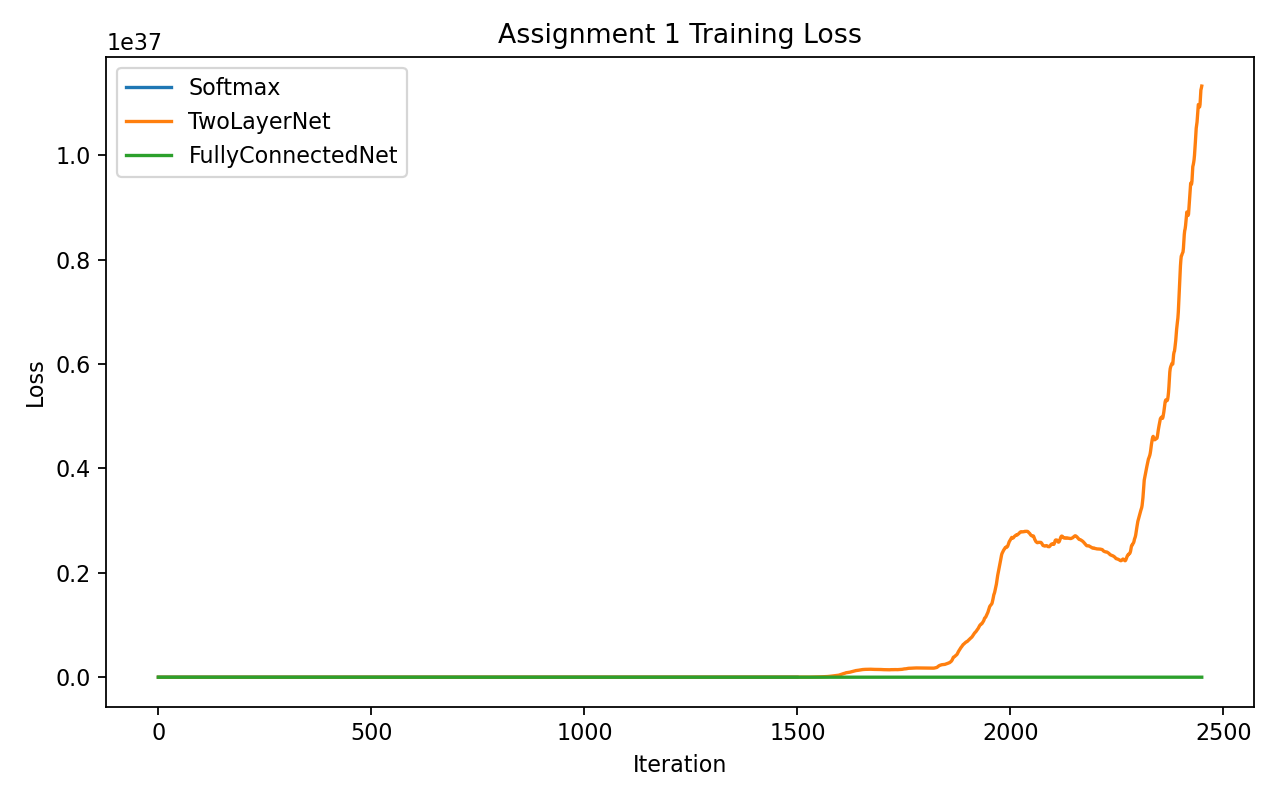
\includegraphics[width=0.84\linewidth]{assignment1_loss_curves.png}
\caption{Assignment 1 baseline 训练损失曲线}
\end{figure}

\begin{figure}[H]
\centering
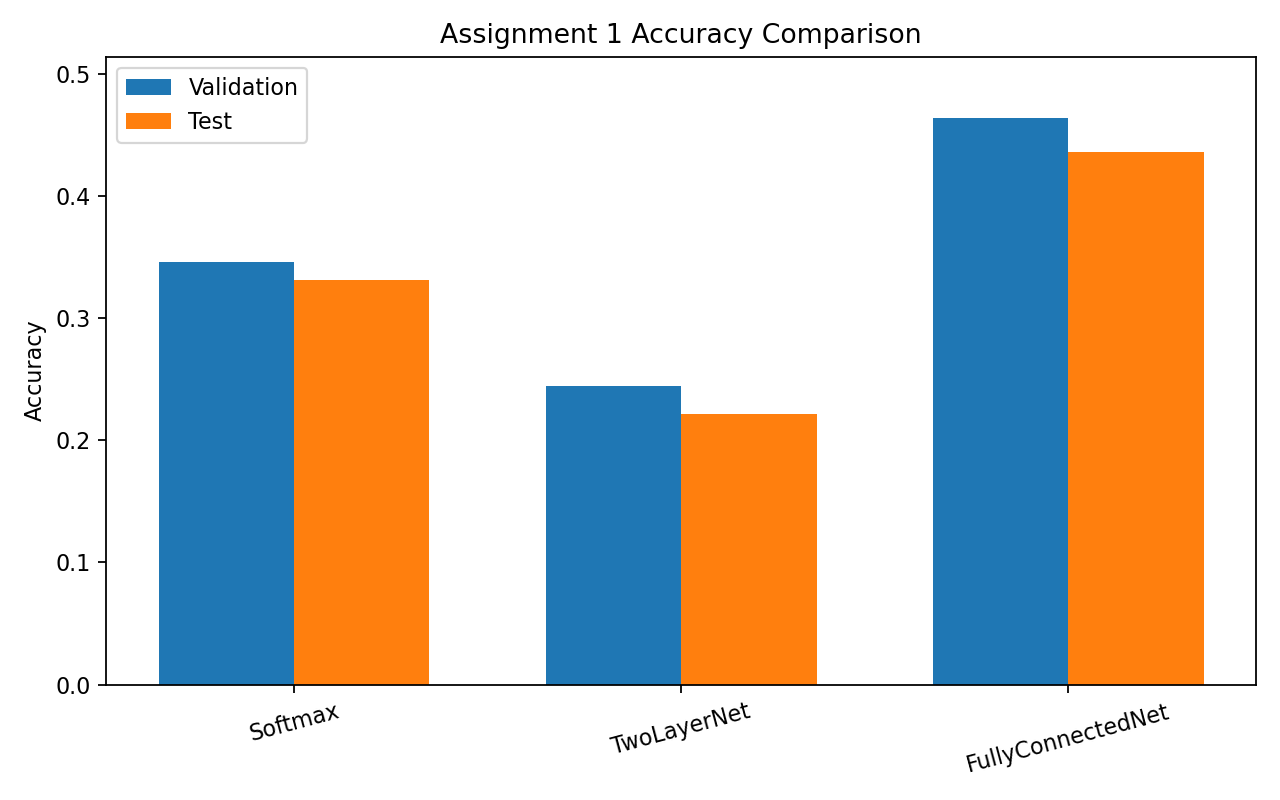
\includegraphics[width=0.84\linewidth]{assignment1_accuracy_comparison_full_data.png}
\caption{Assignment 1 baseline 验证集与测试集准确率对比}
\end{figure}

\subsection{kNN 搜索结果}

\begin{table}[H]
\centering
\begin{tabular}{lccc}
\toprule
方法 & 选择的 $k$ & 验证准确率 & 测试准确率 \\
\midrule
hard search & 1 & 0.3570 & 0.3513 \\
elbow selection & 1 & 0.3570 & 0.3513 \\
\bottomrule
\end{tabular}
\caption{kNN hard search 与 elbow 选择结果}
\end{table}

两个选择策略都落在 $k=1$，说明在完整训练集和当前验证集上，最近邻样本本身提供了最强的局部匹配信号。

\subsection{线性分类器搜索结果}

\begin{table}[H]
\centering
\begin{tabular}{lcccc}
\toprule
实验 & 选中配置 & 训练准确率 & 验证准确率 & 测试准确率 \\
\midrule
Softmax & lr=$10^{-7}$, reg=$10^4$ & 0.3546 & 0.3780 & 0.3523 \\
SVM & lr=$10^{-7}$, reg=$10^4$ & 0.3842 & 0.3860 & 0.3760 \\
\bottomrule
\end{tabular}
\caption{Softmax 与 SVM 搜索结果}
\end{table}

SVM 在完整训练设置下取得测试准确率 0.3760，优于 Softmax 的 0.3523。两者的最佳验证配置都使用较低正则强度 $10^4$，说明在完整训练集上，过强的 L2 约束会限制线性分类器的有效容量。

\subsection{TwoLayerNet 搜索结果}

\begin{table}[H]
\centering
\begin{tabular}{lcccc}
\toprule
实验 & 选中配置 & 训练准确率 & 验证准确率 & 测试准确率 \\
\midrule
学习率搜索 & lr=$10^{-4}$ & 0.5469 & 0.4920 & 0.4802 \\
L2 正则搜索 & reg=$10^{-3}$ & 0.2299 & 0.2370 & 0.2401 \\
batch size 搜索 & batch size=128 & 0.2234 & 0.2400 & 0.2193 \\
\bottomrule
\end{tabular}
\caption{TwoLayerNet 超参数搜索结果}
\end{table}

\begin{table}[H]
\centering
\begin{tabular}{lcccc}
\toprule
配置 & 学习率 & 数值状态 & 验证准确率 & 测试准确率 \\
\midrule
A1-HP-LR-001 & $10^{-2}$ & loss 溢出并出现 NaN & 0.1670 & 0.1533 \\
A1-HP-LR-002 & $10^{-3}$ & loss 放大到 $10^{40}$ 量级 & 0.2280 & 0.2303 \\
A1-HP-LR-003 & $10^{-4}$ & loss 稳定下降 & 0.4920 & 0.4802 \\
\bottomrule
\end{tabular}
\caption{TwoLayerNet 学习率搜索的数值稳定性}
\end{table}

学习率搜索中，$10^{-2}$ 和 $10^{-3}$ 都表现出明显的数值不稳定。前者在训练中出现溢出和 NaN，后者虽然没有变成 NaN，但 final loss 达到 $10^{40}$ 量级，已经不能作为稳定收敛的候选配置。可以 看出，学习率过大导致参数更新越过了 loss landscape 中的稳定区域，造成训练震荡和发散。因此，应合理选择学习率，以充分利用短训练期内的快速迭代。

\subsection{消融实验结果}

\begin{table}[H]
\centering
\begin{tabular}{lcccc}
\toprule
实验 & 选中配置 & 训练准确率 & 验证准确率 & 测试准确率 \\
\midrule
初始化消融 & He 初始化 & 0.2358 & 0.2520 & 0.2318 \\
优化器消融 & SGD & 0.5489 & 0.4960 & 0.4855 \\
归一化/dropout 消融 & 无归一化/无 Dropout & 0.4777 & 0.4840 & 0.4637 \\
\bottomrule
\end{tabular}
\caption{Assignment 1 消融实验结果}
\end{table}

\begin{figure}[H]
\centering
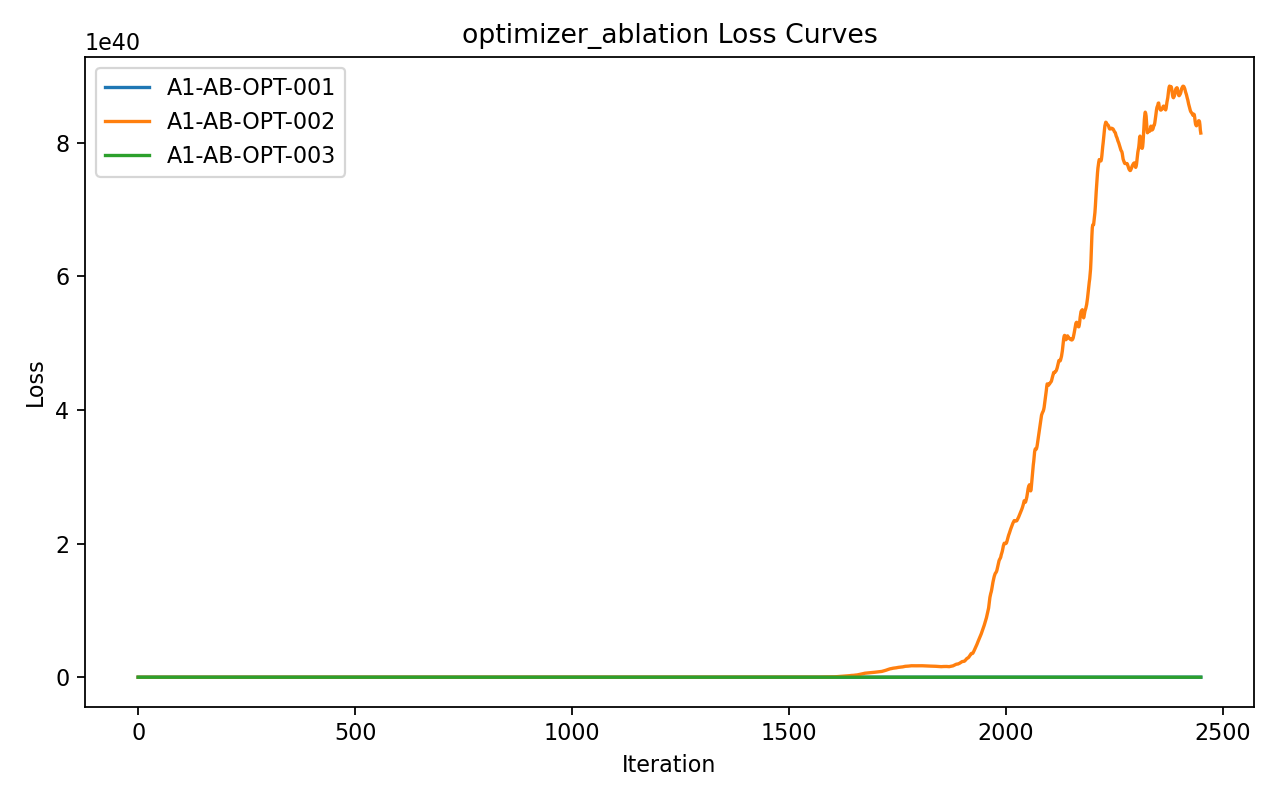
\includegraphics[width=0.84\linewidth]{optimizer_ablation_loss_curves.png}
\caption{优化器消融损失曲线}
\end{figure}

\begin{figure}[H]
\centering
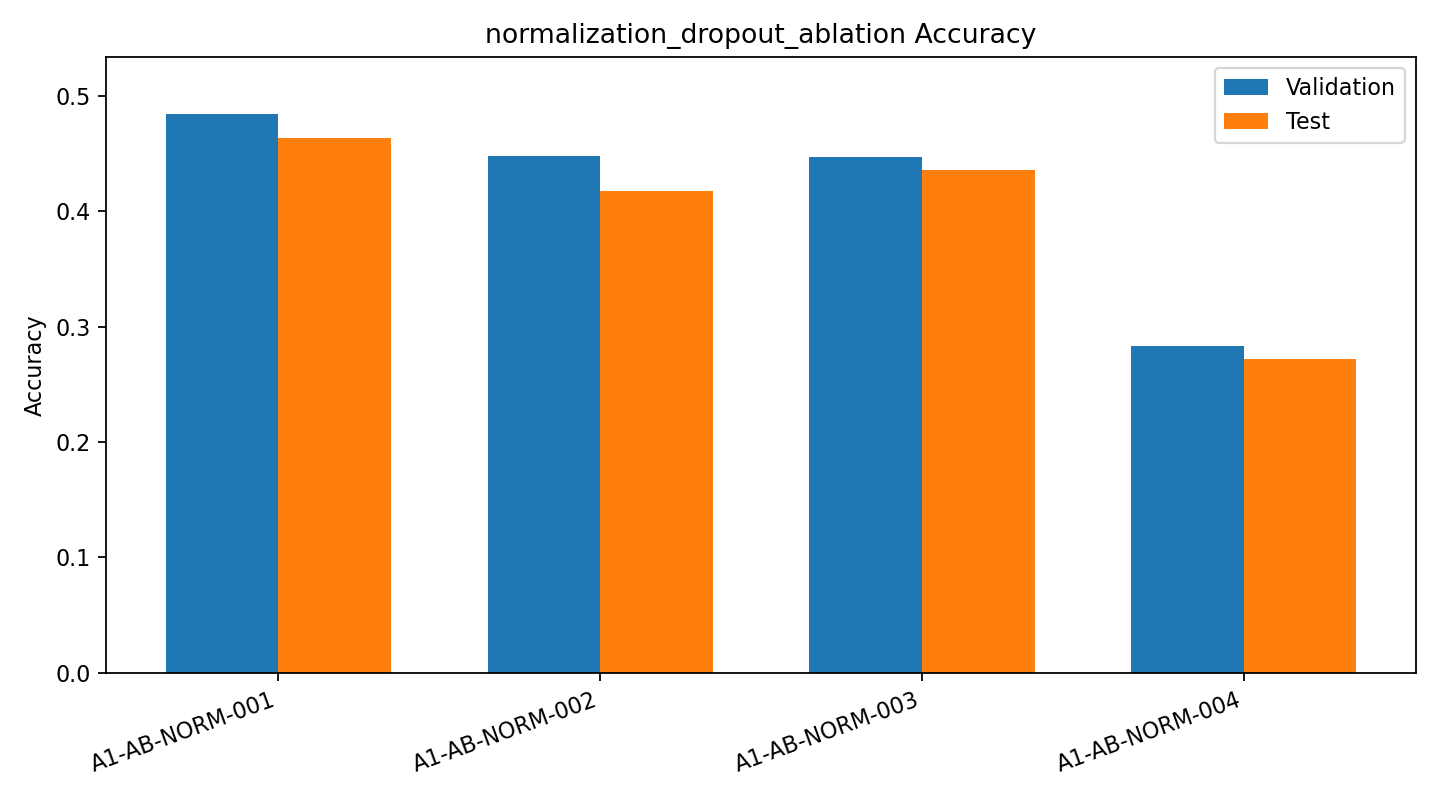
\includegraphics[width=0.84\linewidth]{normalization_dropout_ablation_accuracy.png}
\caption{归一化与 Dropout 消融准确率对比}
\end{figure}

初始化消融中，零初始化接近随机猜测，符合隐藏单元对称性无法有效破缺的预期。He 初始化在固定 $lr=10^{-3}$ 的 momentum 配置下验证准确率略高，但 final loss 偏大，说明初始化方式需要和学习率共同判断。优化器消融中 SGD 取得最高验证和测试准确率，Momentum 在同一学习率下发散，Adam 则稳定但测试准确率低于 SGD。归一化/dropout 消融中，无归一化且不使用 Dropout 的全连接网络表现最好；BatchNorm 和 LayerNorm 在当前浅层、短训练配置下没有带来提升，Dropout 单独使用明显降低容量。

\section{问题、调试过程与解决方案}

\subsection{学习率发散现象}

TwoLayerNet 学习率搜索中，$lr=10^{-2}$ 出现溢出和 NaN，$lr=10^{-3}$ 的 loss 也放大到 $10^{40}$ 量级。这是学习率过大导致参数更新越过稳定区域的典型现象。解决方案是引入学习率衰减机制，或者在搜索过程中增加更细粒度的学习率选项，如 $5\times10^{-4}$、$2\times10^{-4}$ 等，以找到既能快速下降又不失稳定性的学习率。

\section{阶段性总结与后续计划}

\subsection{模型理解方面的收获}

kNN 体现了非参数方法中“训练简单、预测依赖全量距离计算”的特点；Softmax/SVM 体现了线性分类器在原始像素上的基本判别能力；TwoLayerNet 和 FullyConnectedNet 展示了非线性模型容量提升后对学习率、初始化、正则和优化器更敏感。

\subsection{调优能力方面的收获}

本阶段结果说明，调参需要同时看 loss 曲线、验证准确率、测试准确率和 train-val gap。验证集用于选择配置，测试集用于最终观察；当测试表现与验证选择不完全一致时，应优先维护验证集选择原则，避免测试集泄漏到调参过程。

\end{document}
